%Version 3.1 December 2024
% See section 11 of the User Manual for version history
%
%%%%%%%%%%%%%%%%%%%%%%%%%%%%%%%%%%%%%%%%%%%%%%%%%%%%%%%%%%%%%%%%%%%%%%
%%                                                                 %%
%% Please do not use \input{...} to include other tex files.       %%
%% Submit your LaTeX manuscript as one .tex document.              %%
%%                                                                 %%
%% All additional figures and files should be attached             %%
%% separately and not embedded in the \TeX\ document itself.       %%
%%                                                                 %%
%%%%%%%%%%%%%%%%%%%%%%%%%%%%%%%%%%%%%%%%%%%%%%%%%%%%%%%%%%%%%%%%%%%%%

%%\documentclass[referee,sn-basic]{sn-jnl}% referee option is meant for double line spacing

%%=======================================================%%
%% to print line numbers in the margin use lineno option %%
%%=======================================================%%

%%\documentclass[lineno,pdflatex,sn-basic]{sn-jnl}% Basic Springer Nature Reference Style/Chemistry Reference Style

%%=========================================================================================%%
%% the documentclass is set to pdflatex as default. You can delete it if not appropriate.  %%
%%=========================================================================================%%

%%\documentclass[sn-basic]{sn-jnl}% Basic Springer Nature Reference Style/Chemistry Reference Style

%%Note: the following reference styles support Namedate and Numbered referencing. By default the style follows the most common style. To switch between the options you can add or remove “Numbered” in the optional parenthesis. 
%%The option is available for: sn-basic.bst, sn-chicago.bst%  
 
%%\documentclass[pdflatex,sn-nature]{sn-jnl}% Style for submissions to Nature Portfolio journals
%%\documentclass[pdflatex,sn-basic]{sn-jnl}% Basic Springer Nature Reference Style/Chemistry Reference Style
\documentclass[pdflatex,sn-mathphys-num]{sn-jnl}% Math and Physical Sciences Numbered Reference Style
%%\documentclass[pdflatex,sn-mathphys-ay]{sn-jnl}% Math and Physical Sciences Author Year Reference Style
%%\documentclass[pdflatex,sn-aps]{sn-jnl}% American Physical Society (APS) Reference Style
%%\documentclass[pdflatex,sn-vancouver-num]{sn-jnl}% Vancouver Numbered Reference Style
%%\documentclass[pdflatex,sn-vancouver-ay]{sn-jnl}% Vancouver Author Year Reference Style
%%\documentclass[pdflatex,sn-apa]{sn-jnl}% APA Reference Style
%%\documentclass[pdflatex,sn-chicago]{sn-jnl}% Chicago-based Humanities Reference Style

%%%% Standard Packages
%%<additional latex packages if required can be included here>

\usepackage{graphicx}%
\usepackage{multirow}%
\usepackage{amsmath,amssymb,amsfonts}%
\usepackage{amsthm}%
\usepackage{mathrsfs}%
\usepackage[title]{appendix}%
\usepackage{xcolor}%
\usepackage{textcomp}%
\usepackage{manyfoot}%
\usepackage{booktabs}%
\usepackage{algorithm}%
\usepackage{algorithmicx}%
\usepackage{algpseudocode}%
\usepackage{listings}%
\usepackage{wasysym}%
\usepackage{biblatex}
\addbibresource{citations.bib}
%%%%

%%%%%=============================================================================%%%%
%%%%  Remarks: This template is provided to aid authors with the preparation
%%%%  of original research articles intended for submission to journals published 
%%%%  by Springer Nature. The guidance has been prepared in partnership with 
%%%%  production teams to conform to Springer Nature technical requirements. 
%%%%  Editorial and presentation requirements differ among journal portfolios and 
%%%%  research disciplines. You may find sections in this template are irrelevant 
%%%%  to your work and are empowered to omit any such section if allowed by the 
%%%%  journal you intend to submit to. The submission guidelines and policies 
%%%%  of the journal take precedence. A detailed User Manual is available in the 
%%%%  template package for technical guidance.
%%%%%=============================================================================%%%%

%% as per the requirement new theorem styles can be included as shown below
\theoremstyle{thmstyleone}%
\newtheorem{theorem}{Theorem}%  meant for continuous numbers
%%\newtheorem{theorem}{Theorem}[section]% meant for sectionwise numbers
%% optional argument [theorem] produces theorem numbering sequence instead of independent numbers for Proposition
\newtheorem{proposition}[theorem]{Proposition}% 
%%\newtheorem{proposition}{Proposition}% to get separate numbers for theorem and proposition etc.

\theoremstyle{thmstyletwo}%
\newtheorem{example}{Example}%
\newtheorem{remark}{Remark}%

\theoremstyle{thmstylethree}%
\newtheorem{definition}{Definition}%

\raggedbottom
%%\unnumbered% uncomment this for unnumbered level heads

\begin{document}

\title[Lorentz Factor as the Slope of a Fourth Spatial Coordinate]{The Lorentz Factor as the Slope of a Fourth Spatial Coordinate: One Embedding Relation for Schwarzschild, Stellar Interiors, Frame Dragging and the Hubble Flow}

\author*[1]{\fnm{Andrew} \sur{Mueller}}\email{AndrewMueller414@gmail.com}

\affil*[1]{\orgname{Independent Researcher}, \orgaddress{\city{Milwaukee}, \postcode{53219}, \state{WI}, \country{USA}}}

\abstract{We examine what follows if the Lorentz factor is read as the slope of an additional, non-compact spatial coordinate $y$, $\gamma=\sqrt{1+(\partial_xy)^2}$, so that the slope $\gamma\beta=\sinh\eta$ is set by the rapidity $\eta$. For a spherical source the Gauss equation of the embedded slice, together with the time-symmetric Hamiltonian constraint, gives $\beta^2=2Gm(R)/(c^2R)$, where $\beta c$ is the flow velocity of the Painlev\'e--Gullstrand picture. The same relation yields the Flamm paraboloid outside a mass, a spherical cap inside a uniform ball and the Hubble flow of a critical-density universe. In a static region the Gauss equation and the static Einstein equations fix the lapse: $N=\cos\theta=1/\gamma$ in vacuum, and the Tolman--Oppenheimer--Volkoff potential gradient with matter. For a uniform-density ball the lapse is $N=\left(3\cos\theta_*-\cos\theta\right)/2$, and the Buchdahl bound $R_*>9r_s/8$ is the statement that the tilt of the slice at the surface is below $70.5^\circ$. To first order in the angular momentum the non-gradient part of the Kaluza--Klein potential is the vorticity of the flow of space, and the momentum constraint gives the Lense--Thirring solution on the same slice. The metric component $G_{44}$ is fixed to unity, consistent with the Cassini bound. Every result is equivalent to a known result of general relativity, whose field equations are imported and not derived here. The contribution is a single geometric picture with explicit checks, and a statement of what remains open.}

\keywords{embedding diagrams, Painlev\'e--Gullstrand coordinates, Buchdahl bound, Lense--Thirring effect, Kaluza--Klein theory}

\maketitle

\section{Introduction}\label{sec_intro}

Embedding diagrams are a standard way to picture the spatial geometry of a gravitational field. The Flamm paraboloid shows the spatial slice of the Schwarzschild solution as a surface in flat space~\cite{Flamm1916}, and a spherical cap shows the interior of a uniform ball~\cite{Schwarzschild1916}. A second standard picture treats space as a flat background that flows past observers: the Painlev\'e--Gullstrand form of the Schwarzschild metric~\cite{Painleve1921,Gullstrand1922,MartelPoisson2001} and the river model built on it~\cite{HamiltonLisle2008}. These are usually presented as separate devices. Here we ask how much of this structure is a single relation, if one starts from the Lorentz factor.

The starting point is elementary. For a body moving with speed $v=\beta c$ the Lorentz factor $\gamma$ and the quantity $\gamma\beta$ satisfy $\gamma^2=1+(\gamma\beta)^2$. If $\gamma\beta$ is read as the slope $\partial_xy$ of a surface in an additional spatial coordinate $y$, then $\gamma=\sqrt{1+(\partial_xy)^2}$, and the identity is the hyperbolic relation $\cosh^2\eta=1+\sinh^2\eta$ for the rapidity $\eta$. Non-compact fifth dimensions are not new: in induced-matter theory the fifth coordinate is left unrestricted~\cite{Wesson1999,OverduinWesson1997}, and the Campbell--Magaard theorem~\cite{Campbell1926,Magaard1963} guarantees that any (analytic) solution of the four-dimensional Einstein equations embeds locally in a five-dimensional Ricci-flat space. The difference here is that $y$ is fixed kinematically by the Lorentz factor, not by field equations, and that the construction is applied to the spatial slice.

We show that the following results then follow from one geometric relation, with the inputs from general relativity stated explicitly in each case.
\begin{enumerate}
\item For a spherical source, the Gauss equation and the time-symmetric Hamiltonian constraint give $\beta^2=2Gm(R)/(c^2R)$, so that $\beta c$ is the escape velocity from the enclosed mass (section~\ref{sec_slice}). The exterior of a mass, a uniform ball and a critical-density universe are three cases of this relation.
\item The lapse is not an additional assumption in a static region. In vacuum, the angular component of the static Einstein equations gives $N=1/\gamma=\cos\theta$, where $\theta$ is the tilt of the slice (section~\ref{sec_lapse}). With matter, it gives the potential gradient of the Tolman--Oppenheimer--Volkoff equation.
\item For a uniform-density ball the lapse and pressure have closed forms, and the Buchdahl bound $R_*>9r_s/8$ is the statement that the surface tilt is below $70.5^\circ$ (section~\ref{sec_lapse}).
\item Infall onto a mass and the Hubble expansion are the same relation with opposite sign of the flow (section~\ref{sec_flows}).
\item To first order in the angular momentum $J$, the non-gradient part of the Kaluza--Klein potential is the vorticity of the flow, and the momentum constraint on the same slice gives the Lense--Thirring solution (section~\ref{sec_rotation}).
\item The extra metric component $G_{44}$ is fixed to unity and agrees with the Cassini bound (section~\ref{sec_scalar}).
\end{enumerate}

\paragraph{Scope.} Each result is equivalent to a known result of general relativity, and this paper makes no claim of different predictions. The static Einstein equations, the Hamiltonian constraint and the momentum constraint are imported, not obtained from a five-dimensional action, and the extra coordinate has no independent dynamics here. What is offered is a single geometric reading, with explicit checks (appendix~\ref{sec_checks}), that connects the Lorentz factor, the Flamm embedding, the flow picture, the lapse and the Buchdahl bound. Speculative extensions of this programme are deliberately not included: a reinterpretation of simultaneity, the removal of time as a dimension, a hypothesis about inertia at low accelerations, and numerical coincidences involving Solar-System quantities.

\section{The Lorentz Factor as a Slope}\label{sec_slope}

\subsection{Construction}

Consider a body moving with speed $v$, $\beta=v/c$, $\gamma=\left(1-\beta^2\right)^{-1/2}$. Let $dx=v\tau$ be the ordinary spatial displacement during a parameter interval $\tau$, and let $dx^{(U)}=\gamma\,dx$ be the extended displacement, the Lorentz-dilated separation. We represent the difference by an additional spatial coordinate $y$, orthogonal to the three ordinary ones, so that $dx$, $dy$ and $dx^{(U)}$ form the right triangle of figure~\ref{fig_triangle}:

\begin{equation}\label{eq_pythagoras}
    \left(dx^{(U)}\right)^2=dx^2+dy^2 .
\end{equation}
Solving for $dy$,
\begin{equation}\label{eq_dy}
    dy=v\tau\sqrt{\gamma^2-1}=\tau\,\frac{v^2}{\sqrt{c^2-v^2}} .
\end{equation}

\begin{figure}[t]
\centering
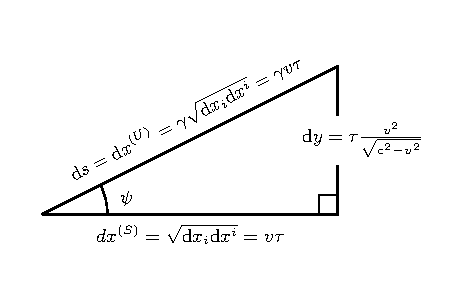
\includegraphics[width=0.6\textwidth]{../diagrams/outputs/simple_triangle.eps}
\caption{Right-triangle construction: the ordinary spatial displacement $dx$, the additional displacement $dy$ and the extended displacement $dx^{(U)}$. The relation $dx^{(U)}=\gamma\,dx$ for the hypotenuse is the assumption of the construction.}
\label{fig_triangle}
\end{figure}

Along a path $y=y(x)$ the slope of the triangle is
\begin{equation}\label{eq_slope}
    \partial_xy=\sqrt{\gamma^2-1}=\gamma\beta ,
    \qquad\text{so}\qquad
    \gamma=\sqrt{1+\left(\partial_xy\right)^2} .
\end{equation}
The parameter $\tau$ cancels from the slope, so equation~\eqref{eq_slope} contains no unit of time. The angle $\theta$ that the triangle makes with the ordinary axis satisfies
\begin{equation}\label{eq_tilt}
    \tan\theta=\gamma\beta,\qquad \sin\theta=\beta,\qquad \cos\theta=\frac1\gamma .
\end{equation}
In terms of the rapidity $\eta$, $\gamma=\cosh\eta$ and $\gamma\beta=\sinh\eta$, so the triangle is the identity $\cosh^2\eta=1+\sinh^2\eta$. Nothing new is asserted by this algebra. The content lies in reading $\gamma\beta$ as the slope of a surface, which is what the gravitational applications below use.

\subsection{Consistency with the Lorentz transformation}

Take an event separated from the origin of a frame $S$ by a purely spatial displacement $dx$, so $dt=0$. In a frame $S'$ moving with speed $v$ along the displacement, the Lorentz transformation gives
\begin{equation}\label{eq_boost}
    dx'=\gamma\,dx,\qquad c\,dt'=-\gamma\beta\,dx=-\partial_xy\,dx=-dy .
\end{equation}
The Minkowski interval is preserved, $-c^2dt'^2+dx'^2=dx^2$. Equation~\eqref{eq_pythagoras} is the same statement with $c\,dt'$ moved to the other side: $dx'^2=dx^2+\left(c\,dt'\right)^2$. For instantaneous separations the additional coordinate is therefore, up to sign, the time-like component of the boosted separation, and the Euclidean right triangle is the Lorentzian invariant rewritten. This is a consistency check and not an independent derivation. For $dt=0$ it contains no information beyond special relativity.

\subsection{What is not claimed}

The identification in equation~\eqref{eq_boost} holds for instantaneous separations. A treatment of finite intervals, of clock synchronization and of the relativity of simultaneity would be needed before the construction could be offered as an alternative formulation of special relativity, and it is not attempted here.

\subsection{Kaluza--Klein form and the four-potential}\label{sec_kk}

The additional coordinate is written in the Kaluza--Klein form~\cite{Kaluza1921,Klein1926}
\begin{equation}\label{eq_kk}
    dS^2=g_{\mu\nu}dx^\mu dx^\nu+G_{44}\left(dy+\mathcal{A}_\mu dx^\mu\right)^2 ,
\end{equation}
invariant under $y\to y+\Lambda(x)$, $\mathcal{A}_\mu\to\mathcal{A}_\mu-\partial_\mu\Lambda$. The slope of section~\ref{sec_slope} supplies a natural candidate for the potential, $\mathcal{A}_\mu\equiv\partial_\mu y$, evaluated in the rest frame of the source where $y=y(\mathbf{x})$ is static. Then $\mathcal{A}_0=0$ and $\mathcal{A}_i=\beta\gamma\,\hat{n}_i$, and three identities follow:
\begin{equation}\label{eq_potential_identities}
    \gamma^2=1+\mathcal{A}_i\mathcal{A}^i,\qquad
    \eta^{\mu\nu}\mathcal{A}_\mu\mathcal{A}_\nu=\gamma^2-1,\qquad
    \mathcal{F}_{\mu\nu}=\partial_\mu\mathcal{A}_\nu-\partial_\nu\mathcal{A}_\mu=0 .
\end{equation}
The last holds because $\mathcal{A}_\mu$ is a pure gradient, so in this sector the potential is pure gauge and carries no field strength. On a temporal surface ($y'=y-y(\mathbf{x})$ constant) equation~\eqref{eq_kk} restricts to $h_{\mu\nu}=g_{\mu\nu}+G_{44}\mathcal{A}_\mu\mathcal{A}_\nu$. For $g_{ij}=\delta_{ij}$ and $G_{44}=1$ this is $h_{ij}=\delta_{ij}+\partial_iy\,\partial_jy$, the metric induced on a hypersurface of flat $\mathbb{R}^4$. A non-gradient part $a_\mu$ added to $\mathcal{A}_\mu$ is the only way for the five-dimensional geometry to carry a field strength; it is treated for a rotating source in section~\ref{sec_rotation}.

\section{Embedding of the Static Slice}\label{sec_slice}

\subsection{Curvature of the embedded slice}

A hypersurface $y(\mathbf{x})$ of flat $\mathbb{R}^4$ has extrinsic curvature $\mathcal{K}_{ij}=\partial_i\partial_jy/\sqrt{1+\mathcal{A}_k\mathcal{A}^k}$, and its intrinsic curvature follows from the Gauss equation, ${}^{(3)}\!R_{ijkl}=\mathcal{K}_{ik}\mathcal{K}_{jl}-\mathcal{K}_{il}\mathcal{K}_{jk}$. For a spherical profile $y(R)$ with $\partial_Ry=\beta\gamma$, the tangent plane is tilted from the $R$-axis by the angle $\theta$ of equation~\eqref{eq_tilt}, with $d\ell=\gamma\,dR$ the proper radial length, so that $\cos\theta=dR/d\ell$. The principal curvatures are the rates at which the tilt changes along each direction:
\begin{equation}\label{eq_principal_curvatures}
    \kappa_\theta=\kappa_\phi=\frac{\sin\theta}{R}=\frac\beta R,
    \qquad
    \kappa_R=\frac{d\theta}{d\ell}=\frac{d\theta}{dR}\frac{dR}{d\ell}=\frac{\beta'}{\cos\theta}\cos\theta=\beta' .
\end{equation}
The sectional curvatures are $\kappa_R\kappa_\theta=\beta\beta'/R$ and $\kappa_\theta\kappa_\phi=\beta^2/R^2$, so in an orthonormal frame
\begin{equation}\label{eq_ricci_components}
    {}^{(3)}\!R_{\hat R\hat R}=\frac{2\beta\beta'}{R},
    \qquad
    {}^{(3)}\!R_{\hat\theta\hat\theta}=\frac{\beta\beta'}{R}+\frac{\beta^2}{R^2},
\end{equation}
and the scalar curvature is
\begin{equation}\label{eq_scalar_curvature}
    {}^{(3)}\!R=\frac{4\beta\beta'}{R}+\frac{2\beta^2}{R^2}=\frac{2}{R^2}\frac{d}{dR}\left(R\beta^2\right).
\end{equation}

\subsection{The Hamiltonian constraint}

For a static configuration the spatial slice is time-symmetric and the Hamiltonian constraint of general relativity reads ${}^{(3)}\!R=16\pi G\rho/c^2$. Combining this with equation~\eqref{eq_scalar_curvature} and integrating from a regular centre gives
\begin{equation}\label{eq_beta_enclosed}
    \beta^2(R)=\frac{2G\,m(R)}{c^2R},
    \qquad
    m(R)=\int_0^R4\pi\rho R'^2\,dR' ,
\end{equation}
so $\beta c$ is the escape velocity from the enclosed mass. The constraint is imported from general relativity. What the embedding adds is its expression through the Hessian of $y$, which ties the density to the second derivative of the fourth coordinate.

\subsection{Three geometries from one relation}\label{sec_three}

Three cases follow from equation~\eqref{eq_beta_enclosed} (figure~\ref{fig_geometries}).
\begin{itemize}
\item \emph{Exterior of a mass} ($m=M$): $\beta^2=r_s/R$ with $r_s=2GM/c^2$, so $\partial_Ry=\sqrt{r_s/(R-r_s)}$ and
\begin{equation}\label{eq_flamm}
    y=\pm2\sqrt{r_s\left(R-r_s\right)}+C ,
    \qquad
    d\ell^2=dR^2+dy^2=\frac{dR^2}{1-r_s/R}.
\end{equation}
This is Flamm's paraboloid~\cite{Flamm1916}, and $d\ell^2$ is the spatial part of the Schwarzschild metric. In vacuum equation~\eqref{eq_scalar_curvature} requires $R\beta^2$ to be constant, so the escape-velocity slope is the only slope that makes the slice scalar-flat.
\item \emph{Uniform density}: $\beta^2=R^2/L^2$ with $L^2=3c^2/(8\pi G\rho)$, so $y=\pm\sqrt{L^2-R^2}+C$, a spherical cap of a three-sphere of radius $L$. This is the spatial geometry of the interior Schwarzschild solution~\cite{Schwarzschild1916}.
\item \emph{Critical density}: $\rho=3H^2/(8\pi G)$ gives $L=c/H$ and $\beta=HR/c$, the Hubble flow. The Schwarzschild radius of a critical-density ball of radius $c/H$ equals $c/H$.
\end{itemize}

\begin{figure}[t]
\centering
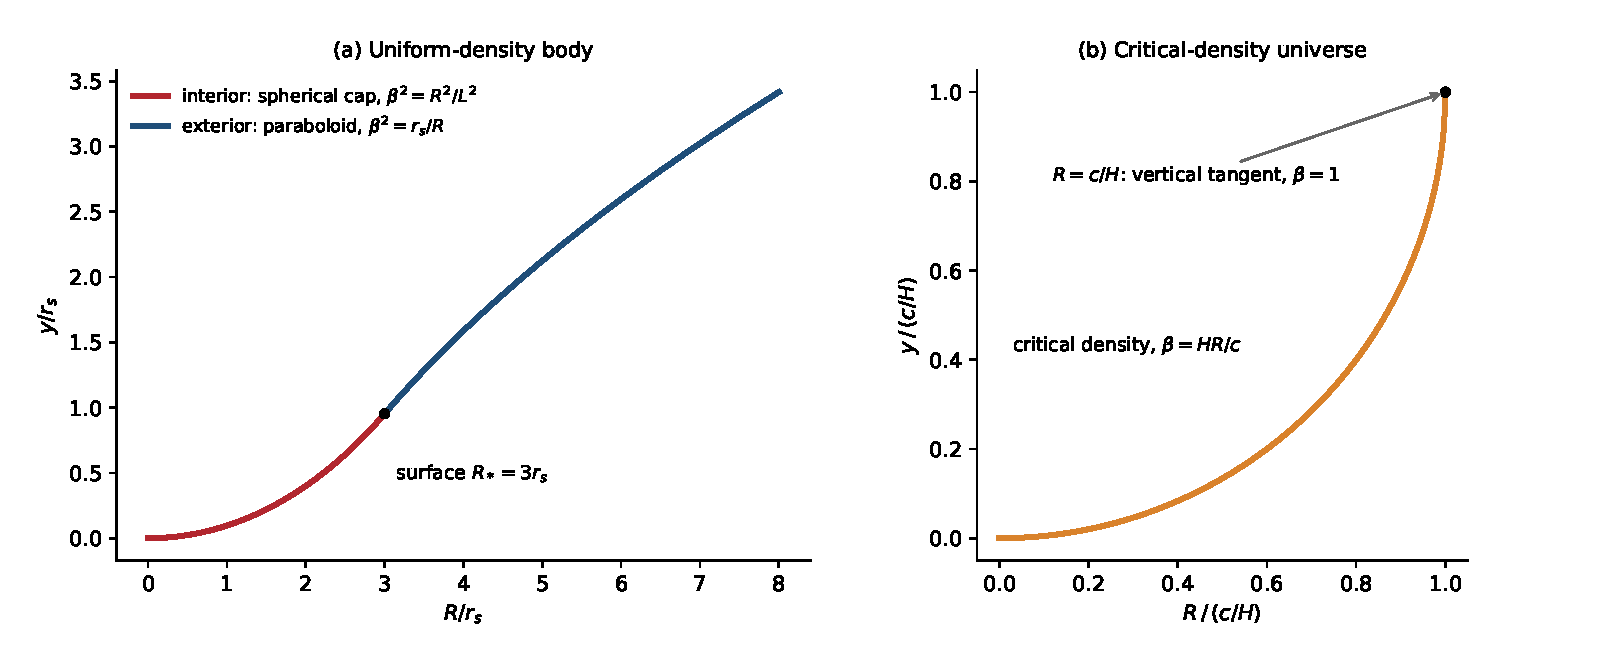
\includegraphics[width=0.95\textwidth]{../diagrams/outputs/embedding_geometries.eps}
\caption{One relation, three embedded profiles. (a)~A uniform-density body of radius $R_*=3r_s$: a spherical cap inside joined to a paraboloid outside. (b)~A critical-density universe, whose profile has a vertical tangent at $R=c/H$.}
\label{fig_geometries}
\end{figure}

\begin{remark}
The real embedding ends where $\beta=1$. At that point the slope $\beta\gamma$ diverges and the tilt reaches $90^\circ$: at the throat $R=r_s$ of the paraboloid and at the Hubble radius $R=c/H$, which is the apparent horizon of the flat universe. For $\beta>1$ the slope is imaginary, and the slice has no real embedding in Euclidean $\mathbb{R}^4$.
\end{remark}

\section{The Lapse}\label{sec_lapse}

Because $\mathcal{A}_0=0$ in the source frame, the embedded slice carries no information about $g_{00}$. The Schwarzschild spacetime is a class-two manifold whose flat embedding is known only in six dimensions~\cite{Kasner1921}, so it cannot be a hypersurface of flat five-dimensional space. The temporal metric function must therefore be supplied separately. The simplest closure is $N=1/\gamma$. This section shows that, in a static region, the closure is not independent: the Gauss equation of the embedding, together with the static Einstein equations, determines $N$.

\subsection{Vacuum}\label{sec_lapse_vacuum}

Write the static metric as $ds^2=-N^2c^2dt^2+h_{ij}dx^idx^j$, with $h_{ij}$ the metric induced on the slice. The vacuum Einstein equations reduce to
\begin{equation}\label{eq_static_vacuum}
    {}^{(3)}\!R_{ij}=\frac1N\nabla_i\nabla_jN,\qquad \Delta N=0 .
\end{equation}
The trace of the first equation is ${}^{(3)}\!R=\Delta N/N$, so together they imply the constraint ${}^{(3)}\!R=0$ already used. With the Gauss equation, ${}^{(3)}\!R_{ij}=\mathcal{K}\,\mathcal{K}_{ij}-\mathcal{K}_{ik}\mathcal{K}^k{}_j$, so the first equation becomes
\begin{equation}\label{eq_lapse_hessian}
    \nabla_i\nabla_jN=N\left(\mathcal{K}\,\mathcal{K}_{ij}-\mathcal{K}_{ik}\mathcal{K}^k{}_j\right).
\end{equation}
The Hessian of the lapse is fixed by the Hessian of the fourth coordinate, and equation~\eqref{eq_lapse_hessian} is a linear equation for $N$ once $y$ is known.

\begin{proposition}\label{prop_lapse}
Let the exterior slice of a static, spherically symmetric vacuum region be the embedding with $\partial_Ry=\beta\gamma$ and $\beta^2=r_s/R$, and let $N\to1$ as $R\to\infty$. Then equation~\eqref{eq_lapse_hessian} implies
\begin{equation}\label{eq_lapse_vacuum}
    N(R)=\sqrt{1-\frac{r_s}{R}}=\frac1\gamma=\cos\theta .
\end{equation}
\end{proposition}

\begin{proof}
In an orthonormal frame the angular Hessian of $N$ is $\nabla_{\hat\theta}\nabla_{\hat\theta}N=\left(R_{,\ell}/R\right)N_{,\ell}$ with $R_{,\ell}=1/\gamma$ and $N_{,\ell}=N'/\gamma$, that is $N'/(\gamma^2R)$. The angular component of equation~\eqref{eq_static_vacuum}, with the curvature of equation~\eqref{eq_ricci_components}, reads
\begin{equation}\label{eq_lapse_ode}
    \frac{N'}{\gamma^2RN}=\frac{\beta\beta'}{R}+\frac{\beta^2}{R^2}
    \quad\Longrightarrow\quad
    \frac{N'}{N}=\gamma^2\left(\beta\beta'+\frac{\beta^2}{R}\right).
\end{equation}
For $\beta^2=r_s/R$ one has $\beta'=-\beta/(2R)$, so $\beta\beta'+\beta^2/R=\beta^2/(2R)$ and
\begin{equation}
    \frac{N'}{N}=\frac{\gamma^2\beta^2}{2R}=\frac{r_s}{2R^2\left(1-r_s/R\right)}=\frac12\frac{d}{dR}\ln\left(1-\frac{r_s}{R}\right).
\end{equation}
Integrating with $N(\infty)=1$ gives the result. The radial component, $N_{,\ell\ell}/N=2\beta\beta'/R$, is then satisfied identically.
\end{proof}

Consequently $g_{00}h_{RR}=-1$ is a theorem of the construction in this region, not an assumption: the redshift factor equals $\cos\theta$, the foreshortening of the embedded slice (figure~\ref{fig_lapse_tilt}).

\begin{figure}[t]
\centering
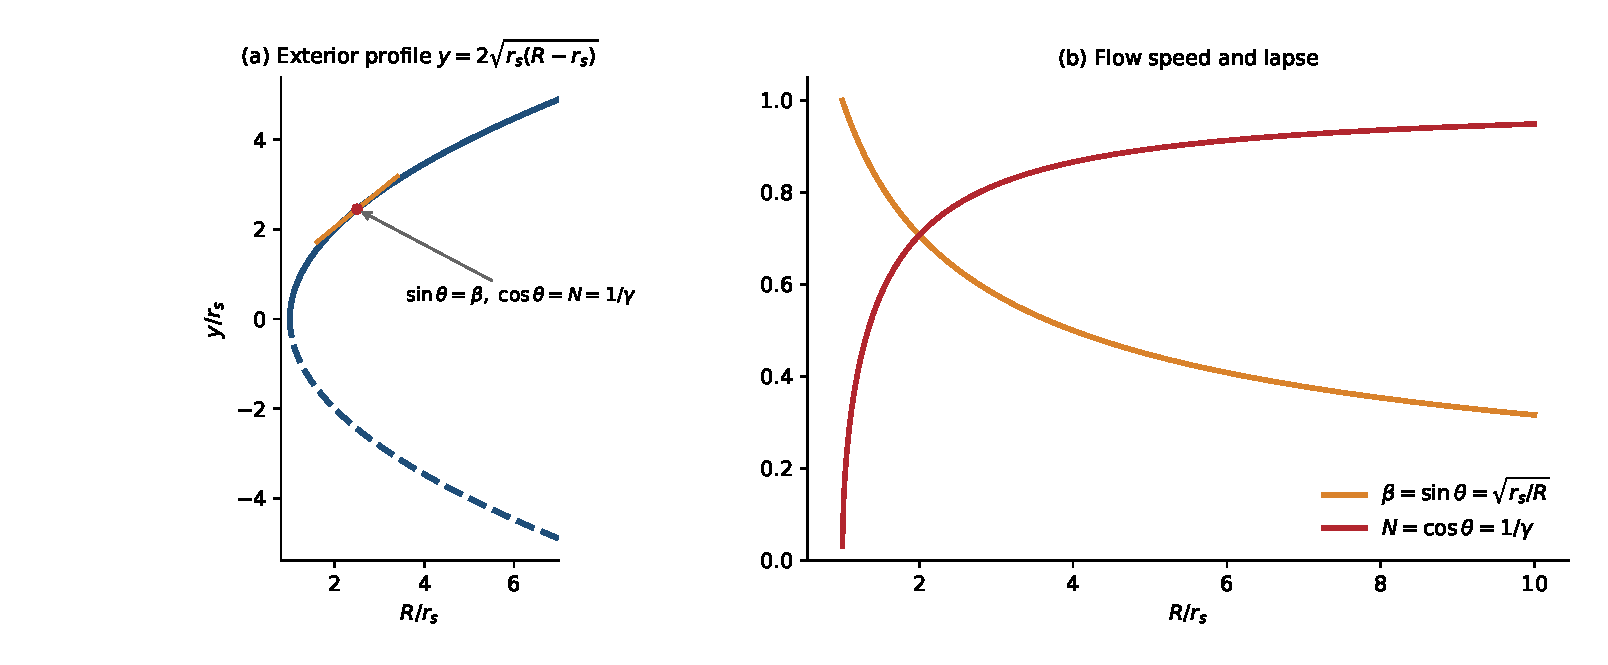
\includegraphics[width=0.95\textwidth]{../diagrams/outputs/lapse_tilt.eps}
\caption{(a)~The exterior profile and the tilt of its tangent, with $\sin\theta=\beta$ and $\cos\theta=N=1/\gamma$. (b)~The flow speed and the lapse as functions of radius.}
\label{fig_lapse_tilt}
\end{figure}

\paragraph{Free fall and marginal binding.} Let $u$ be a radial geodesic with relative Lorentz factor $\gamma_{\rm rel}$ with respect to the static observers. Contracting with the Killing vector $\partial_t$ gives the conserved energy per unit mass, $E=N\gamma_{\rm rel}$. For a body released from rest at infinity $E=1$, hence $\gamma_{\rm rel}=1/N=\gamma$, which is the identification used to define $y$. For a body released from rest at $R_0$, $E=N(R_0)$ and $\gamma_{\rm rel}(R)=N(R_0)/N(R)$, so
\begin{equation}
    \beta_{\rm rel}^2=1-\frac{N(R)^2}{N(R_0)^2}\neq\beta^2 .
\end{equation}
The slope $\beta\gamma$ therefore coincides with $\beta_{\rm rel}\gamma_{\rm rel}$ only for the marginally bound congruence. Bound orbits are described by a different relation between flow and slope, not by a different embedding of the same slice.

\subsection{Matter}\label{sec_lapse_matter}

The slice is unchanged by matter: equation~\eqref{eq_beta_enclosed} holds for any density, so $\beta^2=2Gm(R)/(c^2R)$ and $\gamma^2=1/(1-\beta^2)$. For a static perfect fluid with density $\rho(R)$ and pressure $p(R)$ the static Einstein equations read
\begin{equation}\label{eq_static_fluid}
    {}^{(3)}\!R_{ij}-\frac1N\nabla_i\nabla_jN=\frac{4\pi G}{c^4}\left(\rho c^2-p\right)h_{ij}.
\end{equation}
The angular component, with the embedding values of equation~\eqref{eq_ricci_components} and the identity $\left(R\beta^2\right)'=8\pi G\rho R^2/c^2$, gives
\begin{equation}\label{eq_tov_gradient}
    \frac{N'}{N}=\gamma^2\left(\frac{\beta^2}{2R}+\frac{4\pi G\,p\,R}{c^4}\right)
    =\frac{G\left(m+4\pi R^3p/c^2\right)}{c^2R^2\left(1-2Gm/c^2R\right)} .
\end{equation}
This is the potential gradient of the Tolman--Oppenheimer--Volkoff equation~\cite{Tolman1939,OppenheimerVolkoff1939}. The radial component is then satisfied identically provided
\begin{equation}\label{eq_hydrostatic}
    p'=-\left(\rho c^2+p\right)\frac{N'}{N},
\end{equation}
which is hydrostatic equilibrium. Outside the matter $p=0$ and equation~\eqref{eq_tov_gradient} reduces to the vacuum result. Inside matter $N\neq1/\gamma$: the pressure term adds to the redshift beyond the foreshortening of the slice.

\subsection{Uniform density and the Buchdahl bound}\label{sec_buchdahl}

For $\rho=\text{const}$, $\beta^2=R^2/L^2$ with $L^2=3c^2/(8\pi G\rho)$, and the slice is the spherical cap of section~\ref{sec_three}. Write $s(R)=\cos\theta=1/\gamma=\sqrt{1-R^2/L^2}$ and $s_*=s(R_*)$. Equations~\eqref{eq_tov_gradient} and~\eqref{eq_hydrostatic} are solved by
\begin{equation}\label{eq_uniform_interior}
    N(R)=\frac{3s_*-s(R)}{2},
    \qquad
    p(R)=\rho c^2\,\frac{s(R)-s_*}{3s_*-s(R)} ,
\end{equation}
with $N(R_*)=s_*=\sqrt{1-r_s/R_*}$ and $p(R_*)=0$. This is the interior Schwarzschild solution~\cite{Schwarzschild1916}. In terms of the tilt of the slice, the interior lapse is $\tfrac32\cos\theta_*-\tfrac12\cos\theta(R)$.

The central pressure is $p_c/\rho c^2=(1-s_*)/(3s_*-1)$, which is finite only for $3s_*>1$. In terms of the slice this means
\begin{equation}\label{eq_buchdahl}
    \gamma_*<3,\qquad\cos\theta_*>\frac13,\qquad\theta_*<\arccos\frac13\simeq70.5^\circ ,
\end{equation}
which is the same as the Buchdahl bound~\cite{Buchdahl1959}
\begin{equation}
    R_*>\frac98\,r_s .
\end{equation}
At the limit the central lapse $N(0)=(3s_*-1)/2$ tends to zero and the central pressure diverges (figure~\ref{fig_interior}). This is derived here only for uniform density. Buchdahl's theorem for any non-increasing density profile~\cite{Buchdahl1959} is not derived in this paper.

\begin{figure}[t]
\centering
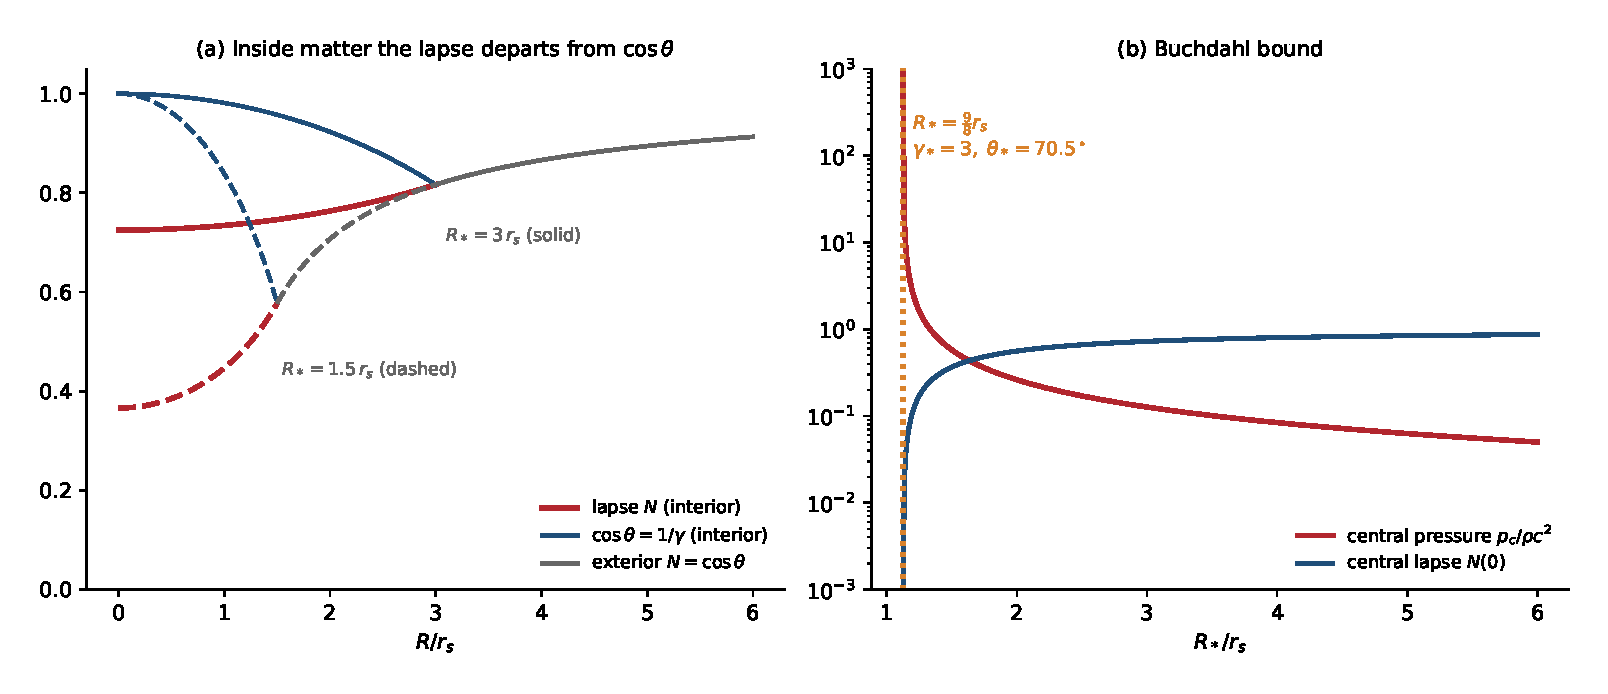
\includegraphics[width=0.95\textwidth]{../diagrams/outputs/interior_lapse.eps}
\caption{(a)~Lapse and slice foreshortening for a uniform-density body, for $R_*=3r_s$ (solid) and $R_*=1.5r_s$ (dashed). Inside matter the lapse is smaller than $\cos\theta$. (b)~Central pressure and central lapse as functions of $R_*/r_s$: the lapse at the centre reaches zero at the Buchdahl limit, where the surface tilt is $70.5^\circ$.}
\label{fig_interior}
\end{figure}

\subsection{Orbits as a corollary}

With the lapse of equation~\eqref{eq_lapse_vacuum} and $A=h_{RR}=\gamma^2$ the static exterior metric is the Schwarzschild metric, and geodesic motion in it is standard (appendix~\ref{sec_orbits}). The circular orbital speed measured by a static observer is $v_{\rm local}^2=c^2R\,N'/N=GM/(R-r_s)$, the angular momentum of a circular orbit is $L^2=GMR^2/(R-3GM/c^2)$, circular orbits exist for $R>3GM/c^2$ and are stable for $R>6GM/c^2$, and the perihelion advance is $\Delta\phi=6\pi GM/\left[a\left(1-e^2\right)c^2\right]$ to leading order. In this framework these are consequences of the embedding together with the derived lapse. They are not independent tests of it.

\section{Flows and Cosmological Expansion}\label{sec_flows}

\subsection{Schwarzschild in Painlev\'e--Gullstrand form}\label{sec_pg}

With $\beta^2=r_s/R$ the Schwarzschild metric can be written~\cite{Painleve1921,Gullstrand1922,MartelPoisson2001}
\begin{equation}\label{eq_pg_metric}
    ds^2=-c^2dT^2+\left(dR+\beta c\,dT\right)^2+R^2d\Omega^2 ,
\end{equation}
where $T$ is the proper time of observers in radial free fall from rest at infinity. The surfaces $T=\text{const}$ are intrinsically flat and $\beta c$ is the Newtonian escape velocity, so space can be pictured as a flat background flowing inward at $\beta c$~\cite{HamiltonLisle2008}. The rest space of an observer held at fixed $R$ has radial metric component
\begin{equation}\label{eq_hrr_flow}
    h_{RR}=g_{RR}-\frac{g_{TR}^2}{g_{TT}}=1+\beta^2\gamma^2=\gamma^2,
    \qquad\gamma=\frac1{\sqrt{1-\beta^2}},
\end{equation}
so $\gamma$ is the Lorentz factor between the infalling frame and the static observers, and the static proper length is $d\ell=\gamma\,dR$. This is the content of equations~\eqref{eq_pythagoras} and~\eqref{eq_dy}, with $x$ the coordinate $R$ of the flat slices, $y$ the Flamm embedding of the static slice, and $\partial_Ry=\beta\gamma$. Along a free-fall worldline $dR/dT=-\beta c$, so $dy/dT=-c\beta^2\gamma$, whose magnitude with $v=\beta c$ is $v^2/\sqrt{c^2-v^2}$, as in equation~\eqref{eq_dy}. The parameter $\tau$ of section~\ref{sec_slope} therefore plays the role of the proper time $T$ of the flow.

For any $\beta(R)$ the change of time $dT=dt+\beta\,dR/\left[c\left(1-\beta^2\right)\right]$ takes equation~\eqref{eq_pg_metric} to
\begin{equation}
    ds^2=-\left(1-\beta^2\right)c^2dt^2+\frac{dR^2}{1-\beta^2}+R^2d\Omega^2 ,
\end{equation}
so $N^2=1/A=1-\beta^2$ with $A=h_{RR}$. The closure $N=1/\gamma$ is therefore equivalent to requiring that the frame moving at $\beta c$ relative to the static observers has unit lapse and flat slices. For pressureless matter this is exact, because the dust frame is geodesic.

\subsection{Hubble flow}

For a flat Friedmann--Lema\^itre--Robertson--Walker universe, the areal radius $R=a(t)r$ gives $a\,dr=dR-HR\,dt$ and
\begin{equation}\label{eq_flrw_flow}
    ds^2=-c^2dt^2+\left(dR-\beta_Hc\,dt\right)^2+R^2d\Omega^2,
    \qquad\beta_H=\frac{HR}{c},
\end{equation}
the same form as equation~\eqref{eq_pg_metric} with the opposite sign of the shift. With $m=\tfrac{4\pi}{3}\rho R^3$ and the Friedmann equation $H^2=8\pi G\rho/3$, $\beta_H^2=2Gm/(c^2R)$. The Hubble radius $R=c/H$ is where $\beta=1$ and $2Gm/c^2=R$, which is the apparent horizon of the flat universe~\cite{Faraoni2011,Faraoni2022}. The Newtonian counterpart is the zero-energy condition of Milne and McCrea~\cite{Milne1934,McCreaMilne1934}: the Hubble velocity equals the escape velocity from the enclosed mass.

\subsection{The general relation}

For spherical, pressureless, marginally bound dust (Lema\^itre--Tolman--Bondi~\cite{Lemaitre1933,Tolman1934,Bondi1947} with zero energy function), $R'\,dr=dR-\dot R\,dt$ with $\dot R^2=2Gm/R$ gives equation~\eqref{eq_pg_metric} with $\beta^2=2Gm(R,T)/(c^2R)$ and $m$ the Misner--Sharp mass~\cite{MisnerSharp1964}. The generalized Painlev\'e--Gullstrand form extends this to pressure~\cite{LaskyLun2006}. Equation~\eqref{eq_beta_enclosed} is the same relation, and Schwarzschild and flat Friedmann--Lema\^itre--Robertson--Walker are two cases of it (table~\ref{table_cases}). Binding and expansion are then one relation applied to different mass distributions, with the sign of the flow distinguishing infall from expansion.

\begin{table}[t]
\caption{Cases of $\beta^2=2Gm/(c^2R)$ with unit lapse and flat slices.}\label{table_cases}
\begin{tabular}{@{}llll@{}}
\toprule
Configuration & $m(R)$ & Flow & Static-slice embedding\\
\midrule
Exterior of a mass $M$ & $M$ & inward & paraboloid\\
Uniform-density ball & $\tfrac{4\pi}{3}\rho R^3$ & inward or outward & cap of a 3-sphere, $L^2=3c^2/8\pi G\rho$\\
Critical density & $\tfrac{4\pi}{3}\rho_cR^3$ & outward & cap with $L=c/H$\\
\botrule
\end{tabular}
\end{table}

\begin{figure}[t]
\centering
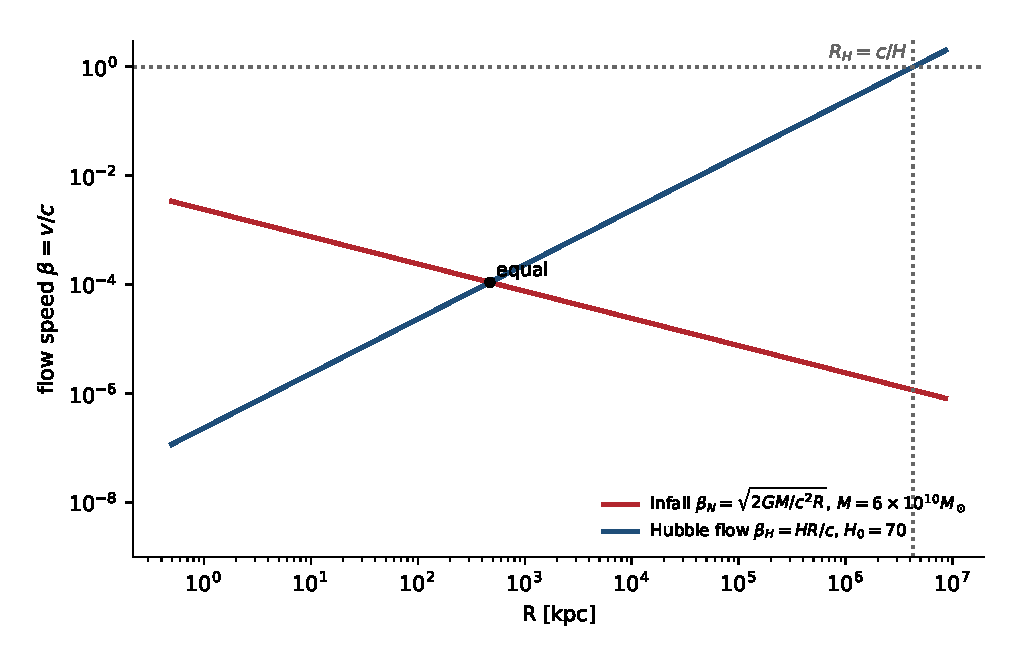
\includegraphics[width=0.7\textwidth]{../diagrams/outputs/flows.eps}
\caption{Infall speed around a Milky-Way-mass body ($6\times10^{10}M_\odot$) and the Hubble flow, as fractions of the speed of light, for $H_0=70~\mathrm{km\,s^{-1}\,Mpc^{-1}}$. The two are equal at about $0.5$ Mpc, and the Hubble flow reaches $\beta=1$ at $R=c/H$.}
\label{fig_flows}
\end{figure}

\subsection{The Sciama--Dicke relation}

At the Hubble radius $\beta_H=1$, so equation~\eqref{eq_flrw_flow} gives
\begin{equation}\label{eq_sciama}
    \frac{G\,m(R_H)}{c^2R_H}=\frac12 ,
    \qquad R_H=\frac cH .
\end{equation}
This is the Sciama--Dicke relation between the mass of the Universe and its size~\cite{Sciama1953}, and here it follows in one line from equation~\eqref{eq_beta_enclosed}. Inside a galaxy the two flows are of very different size (figure~\ref{fig_flows}): for a baryonic mass of $6\times10^{10}M_\odot$ and $H_0=70~\mathrm{km\,s^{-1}\,Mpc^{-1}}$, the ratio of $H_0^2R$ to the Newtonian acceleration $GM/R^2$ is about $10^{-5}$ at $R=8$ kpc and $3\times10^{-4}$ at $25$ kpc, so the Hubble flow is a negligible correction there.

\section{Rotation and the Non-Gradient Component}\label{sec_rotation}

The results above have $a_\mu=0$: a static, spherical source. This section identifies the non-gradient component for a slowly rotating source and shows that, to first order in the angular momentum $J$, it is the gravitomagnetic sector of general relativity. It is an identification and a check, not a new field equation.

\subsection{First order in $J$}

To first order in $J$ rotation changes neither the slice metric $h_{ij}$ nor the lapse $N$. It adds a shift:
\begin{equation}\label{eq_slow_rotation}
    ds^2=-N^2c^2dt^2+\gamma^2dR^2+R^2d\theta^2+R^2\sin^2\theta\left(d\phi-\omega(R)\,dt\right)^2,
    \qquad N=\frac1\gamma ,
\end{equation}
so the embedded slice, with $\partial_Ry=\beta\gamma$, is unchanged. Here $\omega(R)=d\phi/dt$ is the angular velocity of zero-angular-momentum observers, the rate at which space is dragged around the source.

\subsection{Momentum constraint}

For a stationary shift $N^\phi=-\omega$ the extrinsic curvature of the slice in spacetime is $K_{ij}=\left(D_iN_j+D_jN_i\right)/(2Nc)$, and its trace vanishes. This $K_{ij}$ is distinct from the extrinsic curvature $\mathcal{K}_{ij}$ of the embedding in $\mathbb{R}^4$. The vacuum momentum constraint $D_j\!\left(K^{ij}-h^{ij}K\right)=0$ has only a $\phi$-component, which on the slice of this paper is
\begin{equation}\label{eq_momentum_vacuum}
    D_jK^{j\phi}\;\propto\;-\frac{\sqrt{R-r_s}}{R^{9/2}}\,\frac{d}{dR}\!\left(R^4\,\omega'\right)=0 .
\end{equation}
The factors of $r_s$ drop out of the equation $\left(R^4\omega'\right)'=0$, so it is the same as in flat space. With $\omega\to0$ at infinity,
\begin{equation}\label{eq_lt_solution}
    \omega(R)=\frac{2GJ}{c^2R^3},
\end{equation}
which is the Lense--Thirring result~\cite{LenseThirring1918}, here exact on the Flamm slice at this order.

\subsection{Source and the meaning of $J$}

With a momentum density $\rho v^i$ the weak-field constraint reads $\tfrac12\nabla^2N^i=8\pi G\rho v^i/c^2$, so
\begin{equation}\label{eq_shift_poisson}
    N^i(\mathbf{x})=-\frac{4G}{c^2}\int\frac{\rho\,v^i(\mathbf{x}')}{|\mathbf{x}-\mathbf{x}'|}\,d^3x'
    \;\xrightarrow{\;r\to\infty\;}\;
    -\frac{2G}{c^2}\,\frac{(\mathbf{J}\times\mathbf{x})^i}{r^3},
    \qquad
    \mathbf{J}=\int\mathbf{x}\times\rho\mathbf{v}\,d^3x ,
\end{equation}
which is equation~\eqref{eq_lt_solution} with $J$ the usual angular momentum. A numerical integration for a rigidly rotating uniform ball reproduces the far field to five digits (appendix~\ref{sec_checks}).

\subsection{The non-gradient component as vorticity}

The identity $\gamma^2=1+\mathcal{A}_k\mathcal{A}^k$ is satisfied by $\mathcal{A}_i=\gamma\beta_i$, where $\beta_i$ is the velocity of the flow of space relative to the static observers in units of $c$. The radial flow gives the gradient $\partial_Ry$. Rotation adds an azimuthal flow $\mathbf{v}_s=\omega\,\hat{\mathbf{z}}\times\mathbf{x}$, and to leading order in $r_s/R$ this is the non-gradient component,
\begin{equation}\label{eq_nongradient_flow}
    a_i\simeq\frac{v_{s,i}}{c},
    \qquad
    \mathcal{F}=\nabla\times\mathbf{a}=\frac{2GJ}{c^3}\,\frac{3(\hat{\mathbf{z}}\cdot\hat{\mathbf{r}})\hat{\mathbf{r}}-\hat{\mathbf{z}}}{R^3}.
\end{equation}
The non-gradient component is the vorticity of the flow, and $\mathcal{F}$ has the form of a dipole field (figure~\ref{fig_dragging}). A gyroscope at rest precesses with half the vorticity of the flow~\cite{HamiltonLisle2008}, $\boldsymbol{\Omega}=\tfrac c2\mathcal{F}$:
\begin{equation}\label{eq_gyro}
    \boldsymbol{\Omega}_{\mathrm{LT}}=\frac{G}{c^2R^3}\left[3(\mathbf{J}\cdot\hat{\mathbf{r}})\hat{\mathbf{r}}-\mathbf{J}\right],
\end{equation}
the standard Lense--Thirring precession: $2GJ/(c^2R^3)$ at the pole and $-GJ/(c^2R^3)$ at the equator. Averaged over a polar orbit of radius $a$ it is $GJ/(2c^2a^3)$. For $J_\oplus=5.86\times10^{33}~\mathrm{kg\,m^2\,s^{-1}}$ and $a=7027$ km this gives about $41~\mathrm{mas\,yr^{-1}}$, consistent within the accuracy of these rounded inputs with the general-relativistic value and with the Gravity Probe B measurement of $37.2\pm7.2~\mathrm{mas\,yr^{-1}}$~\cite{Everitt2011}.

\begin{figure}[t]
\centering
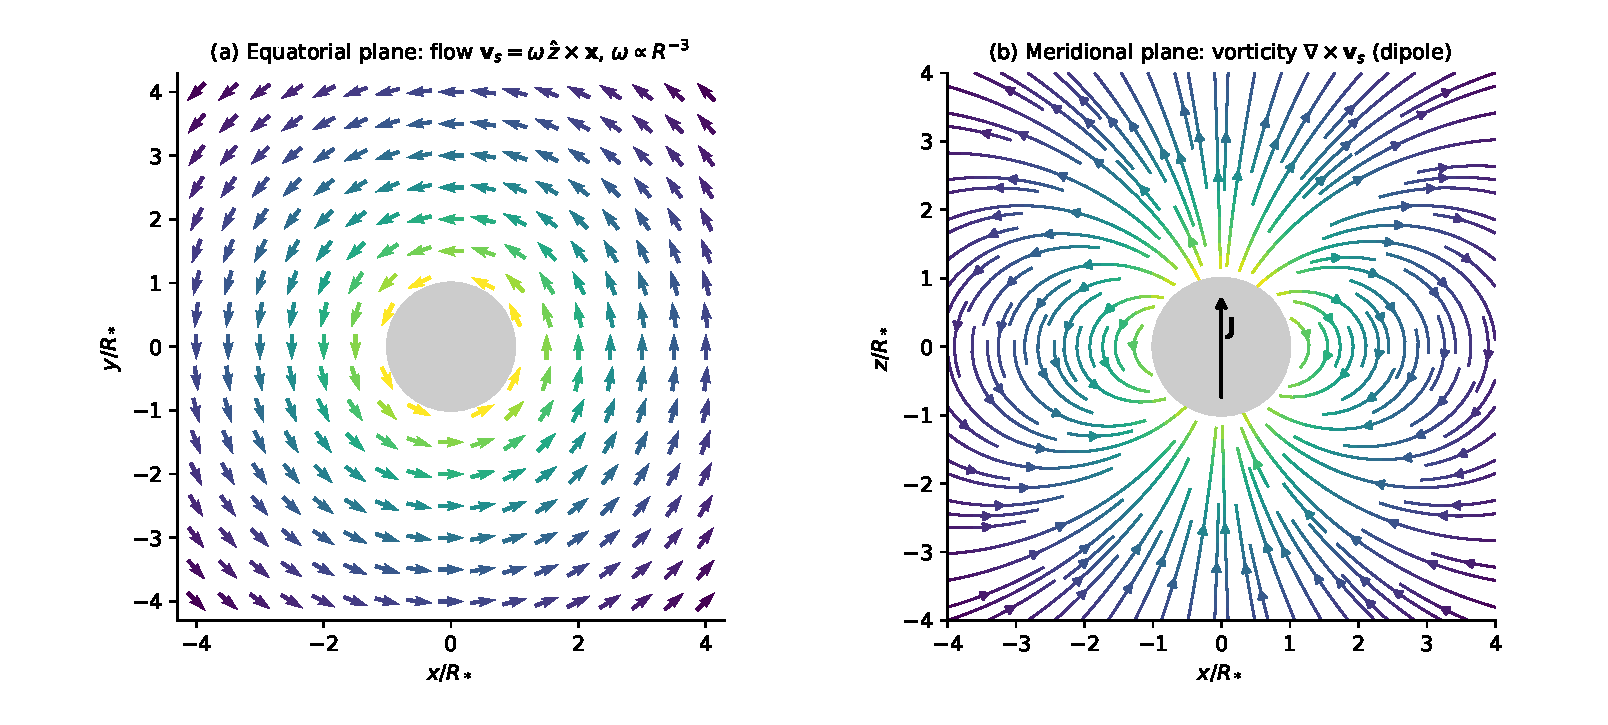
\includegraphics[width=0.95\textwidth]{../diagrams/outputs/frame_dragging.eps}
\caption{(a)~The flow of space $\mathbf{v}_s=\omega\,\hat{\mathbf{z}}\times\mathbf{x}$ in the equatorial plane of a slowly rotating source (arrows normalized, colour showing $\log_{10}|\mathbf{v}_s|$). (b)~The vorticity $\nabla\times\mathbf{v}_s$ in the meridional plane, which has the form of a dipole field and is the non-gradient component $\mathcal{F}$ of equation~\eqref{eq_nongradient_flow}.}
\label{fig_dragging}
\end{figure}

\paragraph{Status.} Derived here: the Lense--Thirring shift on the slice of this paper, the identification of the non-gradient component with the vorticity of the flow, and the gyroscope precession. Imported: the momentum constraint of general relativity. Open: second order in $J$, where $h_{ij}$, $N$ and the embedding change (the Kerr geometry), and the interior frame-dragging equation, which the interior $N$ and $\gamma$ of section~\ref{sec_buchdahl} are sufficient to set up~\cite{Hartle1967}.

\section{The Metric Component $G_{44}$}\label{sec_scalar}

\subsection{Normalization}

For the induced radial metric only the product $G_{44}(dy/dR)^2$ enters,
\begin{equation}
    h_{RR}=1+G_{44}\left(\frac{dy}{dR}\right)^2 ,
\end{equation}
and a rescaling of $y$ absorbs $G_{44}$. Here $y$ is defined kinematically, $dy=v\tau\sqrt{\gamma^2-1}$ (equation~\eqref{eq_dy}), so $\partial_Ry=\beta\gamma$ and $G_{44}$ has a definite value. Requiring the Schwarzschild radial component, $h_{RR}=1/(1-\beta^2)=1+\beta^2\gamma^2$ with $\beta^2=r_s/R$, gives $G_{44}=1$ to all orders in $r_s/R$. To first order the radial component in areal coordinates is $1+\gamma_{\rm PPN}\,r_s/R$, so more generally $G_{44}=\gamma_{\rm PPN}+O(r_s/R)$.

\subsection{Observational bound}

Light deflection and the Shapiro delay scale as $\left(1+\gamma_{\rm PPN}\right)/2$, so $G_{44}$ is measured by these tests. The Cassini radio-link measurement gives $\gamma_{\rm PPN}-1=(2.1\pm2.3)\times10^{-5}$~\cite{Bertotti2003}, hence
\begin{equation}
    G_{44}-1=(2.1\pm2.3)\times10^{-5}
\end{equation}
at $1\sigma$, consistent with $G_{44}=1$. In standard terms a non-constant $G_{44}=\Phi^2$ is a Brans--Dicke-type scalar~\cite{BransDicke1961,OverduinWesson1997}, with $\gamma_{\rm PPN}=(1+\omega_{\rm BD})/(2+\omega_{\rm BD})$. The Cassini measurement then corresponds to $\omega_{\rm BD}\gtrsim4\times10^4$, the bound usually quoted for it~\cite{Bertotti2003}.

\subsection{Vacuum field equation}

Take the five-dimensional vacuum condition, imported here as an assumption, with a static spherical base metric (Schwarzschild) and $G_{44}=\Phi(R)^2$ independent of $y$. The $yy$ component of the Ricci tensor is $R_{yy}=-\Phi\,\Box\Phi$, so
\begin{equation}
    \frac1{R^2}\frac{d}{dR}\!\left[R^2\left(1-\frac{r_s}{R}\right)\frac{d\Phi}{dR}\right]=0
    \quad\Rightarrow\quad
    \Phi=\Phi_\infty\left[1+q\ln\left(1-\frac{r_s}{R}\right)\right].
\end{equation}
The constant $q$ is a scalar charge. The profile diverges logarithmically at $R=r_s$, so regularity at the horizon requires $q=0$ and $G_{44}$ is constant. For a material body the exterior solution occupies $R\ge R_*>r_s$ and the regularity argument does not apply automatically: the scalar charge is then fixed by matching to a sourced interior equation, which is outside the scope of this paper.

\section{Discussion}\label{sec_discussion}

\subsection{What is derived, and what is imported}

Table~\ref{table_status} lists each result of this paper together with the input from general relativity that it relies on.

\begin{table}[t]
\caption{Status of the results.}\label{table_status}
\begin{tabular}{@{}p{0.34\textwidth}p{0.3\textwidth}p{0.3\textwidth}@{}}
\toprule
Result & Imported input & Known result recovered\\
\midrule
$\gamma=\sqrt{1+(\partial_xy)^2}$ & none (algebra) & $\cosh^2\eta=1+\sinh^2\eta$\\
$\beta^2=2Gm/(c^2R)$ & Hamiltonian constraint & Flamm; interior cap; Hubble flow\\
$N=\cos\theta=1/\gamma$ in vacuum & static vacuum Einstein equations & Schwarzschild lapse\\
$N'/N$ with pressure; uniform-density interior & static fluid equations & TOV; interior Schwarzschild\\
$\theta_*<70.5^\circ$ (uniform density) & as above & Buchdahl bound\\
Lense--Thirring shift; non-gradient part as vorticity & momentum constraint & Lense--Thirring; gyroscope precession\\
$G_{44}=1$ & Schwarzschild radial metric & $\gamma_{\rm PPN}=1$; Cassini\\
\botrule
\end{tabular}
\end{table}

\subsection{Relation to general relativity}

Where the construction can be checked it is general relativity in a different representation: the same solutions, with the slope of the fourth coordinate identified with the flow velocity of the Painlev\'e--Gullstrand picture. It makes no prediction that differs from general relativity. Predictions that did differ would have to come from sectors outside the regimes treated here: a non-gradient potential beyond first order in rotation, a varying $G_{44}$, or dynamics of the extra coordinate.

\subsection{Open problems}

\begin{itemize}
\item \emph{A five-dimensional action.} The Hamiltonian constraint, the momentum constraint and the lapse equation are imported. A closed theory would obtain all three from one action. Where such an action allowed $G_{44}\neq1$ or $a_\mu\neq0$, equation~\eqref{eq_lapse_hessian} would acquire extra terms, and those terms would be the candidate source of any departure from general relativity.
\item \emph{Rotation beyond first order.} At second order in $J$ the slice metric, the lapse and the embedding change (the Kerr geometry), and the interior frame-dragging equation has not been solved on this slice.
\item \emph{Time-dependent sources.} The flat slices of the Painlev\'e--Gullstrand form handle marginally bound dust (section~\ref{sec_flows}), but the embedding of the static slice is a static construction. Dynamical collapse and non-marginal cases have not been treated.
\item \emph{The matter-sourced scalar.} A sourced equation for $G_{44}=\Phi^2$ with a fifth-dimensional stress and its consequences for the post-Newtonian parameters are outside the scope of this paper.
\item \emph{Horizons.} The real embedding ends at $\beta=1$ (section~\ref{sec_three}). The continuation of the fourth coordinate beyond this point, where the slope is imaginary, has not been studied.
\item \emph{Simultaneity.} The construction of section~\ref{sec_slope} reproduces the Lorentz transformation for instantaneous separations. Whether it supports an alternative account of finite intervals and clock synchronization is not established.
\end{itemize}

\subsection{Conclusion}

The Lorentz factor can be read as the slope of a fourth spatial coordinate, and the same reading, applied to the spatial slice of a static source, links the Flamm embedding, the flow picture, the gravitational redshift, the TOV equation and the Buchdahl bound, the Hubble flow, and the Lense--Thirring effect through the single relation $\beta^2=2Gm/(c^2R)$ and its first-order rotational extension. The reading is geometric and equivalent to general relativity. It may be useful as a unified way of presenting these standard results, and its value as more than that depends on the open problems above.

\begin{appendices}

\section{Symbolic and Numerical Checks}\label{sec_checks}

The algebra in sections~\ref{sec_slice}--\ref{sec_rotation} was checked with the scripts listed below, supplied with the manuscript as supplementary files. Each script prints the quantity it verifies.
\begin{itemize}
\item \texttt{lapse\_vacuum\_check.py}: the principal curvatures $\kappa_R=\beta'$ and $\kappa_\theta=\beta/R$, the scalar curvature of equation~\eqref{eq_scalar_curvature}, the angular equation~\eqref{eq_lapse_ode}, the integral $N=\sqrt{1-r_s/R}$ and the identical satisfaction of the radial equation (Proposition~\ref{prop_lapse}).
\item \texttt{interior\_lapse\_check.py}: the angular static equation with a fluid reduces to equation~\eqref{eq_tov_gradient}, and the radial equation holds identically given hydrostatic equilibrium~\eqref{eq_hydrostatic}.
\item \texttt{uniform\_star.py}: the closed forms of equation~\eqref{eq_uniform_interior} satisfy both equations, match the exterior at the surface, and give the central pressure and the Buchdahl limit of equation~\eqref{eq_buchdahl}.
\item \texttt{frame\_dragging\_check.py}: the momentum constraint on the Flamm slice reduces to $\left(R^4\omega'\right)'=0$, $\omega=C/R^3$ solves it, and the other components vanish identically.
\item \texttt{weak\_field\_check.py}: the Poisson solution of equation~\eqref{eq_shift_poisson} for a rigidly rotating uniform ball reproduces the far field $-(2G/c^2)(\mathbf{J}\times\mathbf{x})/r^3$ at three radii (ratio $1.00000$); the gyroscope precession of equation~\eqref{eq_gyro} has the stated pole and equator values; and the polar-orbit average for the inputs of section~\ref{sec_rotation} is $40.8~\mathrm{mas\,yr^{-1}}$.
\end{itemize}

\section{Orbits from the Lapse}\label{sec_orbits}

This appendix collects the standard geodesic results used in section~\ref{sec_lapse}. Consider the static metric $ds^2=-N(R)^2c^2dt^2+A(R)\,dR^2+R^2d\phi^2$ in the equatorial plane, with $N^2=1/A=1-r_s/R$. For a massive particle with proper time $\tau_p$ as the affine parameter, the conserved quantities are $E=N^2c^2\dot t$ and $L=R^2\dot\phi$, and the normalization $g_{\mu\nu}\dot x^\mu\dot x^\nu=-c^2$ gives
\begin{equation}
    N^2A\,\dot R^2+V_{\rm eff}(R)=\frac{E^2}{c^2},\qquad V_{\rm eff}=N^2\left(c^2+\frac{L^2}{R^2}\right).
\end{equation}
\paragraph{Circular orbits.} The radial geodesic equation at $\dot R=\ddot R=0$ gives $\Omega^2=d\phi^2/dt^2=c^2NN'/R$. A static observer's proper time is $d\tau_{\rm static}=N\,dt$, so the locally measured speed is
\begin{equation}
    v_{\rm local}^2=\frac{R^2}{N^2}\Omega^2=c^2R\,\frac{N'}{N}=\frac{GM}{R-r_s}.
\end{equation}
Setting $dV_{\rm eff}/dR=0$ gives $L^2=c^2R^3\left(N^2\right)'/\left[2N^2-R\left(N^2\right)'\right]$, which for the Schwarzschild lapse is $L^2=GMR^2/(R-3GM/c^2)$, so circular orbits exist for $R>3GM/c^2$. The second derivative, $V_{\rm eff}''=2c^2r_s(R-3r_s)/\left[R^3(2R-3r_s)\right]$, is positive for $R>3r_s=6GM/c^2$, so the innermost stable circular orbit is at $6GM/c^2$.
\paragraph{Perihelion advance.} With $u=1/R$, $\dot R=-Lu'$ and the first integral above,
\begin{equation}
    L^2\left(u'\right)^2=\frac{E^2}{c^2}-\left(1-r_su\right)\left(c^2+L^2u^2\right),
\end{equation}
and differentiating with respect to $\phi$ gives
\begin{equation}
    \frac{d^2u}{d\phi^2}+u=\frac{GM}{L^2}+\frac{3GM}{c^2}u^2 .
\end{equation}
The first term on the right is Newtonian. With semilatus rectum $p=L^2/GM$ and to first order in $GM/(pc^2)$, the solution is $u\simeq p^{-1}\left[1+e\cos\left((1-3GM/pc^2)\phi\right)\right]$, so the perihelion advances by $\Delta\phi=6\pi GM/(pc^2)=6\pi GM/\left[a(1-e^2)c^2\right]$ per orbit.

\end{appendices}

\bmhead{Competing Interests}
The author declares that there are no competing financial or non-financial interests that could have influenced the work presented in this paper.

\bmhead{Funding}
This research received no external funding.

\bmhead{Author Contributions}
The author conceived, developed, conducted, and wrote this research independently.

\bmhead{Data and Code Availability}
No new datasets were generated or analyzed during this study. The symbolic and numerical checks described in appendix~\ref{sec_checks} are supplied as supplementary scripts.

\bmhead{Ethics Approval}
This research did not involve human participants, animal subjects, or personally identifiable data. Ethics approval was therefore not required.

\bibliography{citations.bib}% common bib file

\end{document}
